\section{Understanding of cache coherence in single core}

Before we determine and analyze MESIF protocol, there are a few important concept
about read-write memory transaction in both single core or multiple cores. To understand
coherence, suppose that we are executing a single core algorithm $S$ on x86 machine and the task
that is sent to processor is to either read or write value to cache at address $A$ where $A$ is 
an arbitrary hexadecimal number. For reading memory by $S$ algorithm, the task is scheduled by CPU 
with read instruction on address $A$ at local cache. Then, the cache on the core is being searched according to
the read instruction and return the value od address $A$ that is currently stored in the cache line as shown in the
figure \ref{fig:read_single_core}.
\begin{figure}[h]
        \centering
        
\includegraphics[width=1\textwidth,scale=0.5]{read_single_core_coherence.png}
        \caption{\label{fig:read_single_core} Read access on cache line}
\end{figure}

Same thing goes the same way with write access on cache. In order to write data into a cache line in a 
particular core, the task of $S$ is being scheduled on core and CPU performs write instruction to address $A$
specify by algorithm $S$ and finish with callback. But, the value on algorithm $S$ will be not be automatically 
update which the algorithm require another read instruction to the same address to retrieve a value as shown in 
figure \ref{fig:write_single_core}. This is also the reason why writing value to cache takes more CPU cycle than read 
in general on both single core and multiple cores. Overall, the timeline of accessing will be write and read repeatedly. 
In single score, everything seems perfectly fine with the design.
Once we run same algorithm in more than 1 processor, there are a drop on performance on accessing cache and memory which will
be determined in the next section.
\begin{figure}[h]
        \centering
        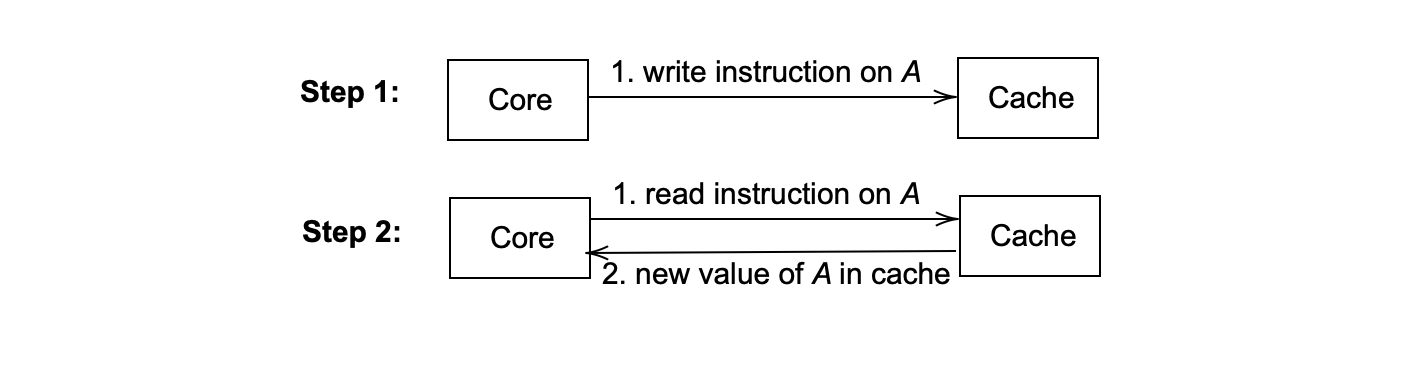
\includegraphics[width=1\textwidth,scale=0.5]{write_single_score_coherence.png}
        \caption{\label{fig:write_single_core} Write access on cache line}
\end{figure}

\section{Understanding of cache coherence in multiple cores}